% ===========================================================================
% An Infrastructure-Constrained, Observation-Evaluated Inventory of
% Oil and Gas Fugitive Emissions in Pakistan
%
% Target journal: Environmental Modelling & Software (Elsevier)
% Document class: elsarticle, 5p layout
% ===========================================================================

\documentclass[5p,times,authoryear]{elsarticle}

% ===========================================================================
% Shared preamble for every manuscript in this repository.
%
% Papers using it:
%   paper/            agriculture inventory
%   paper_nowcast/    agricultural nowcasting
%   paper_national/   the nine-sector national inventory
%   notes/<sector>/   one data note per non-agriculture sector
%
% It exists because paper/ and paper_nowcast/ began as copies of one another
% and had already drifted five lines apart before a third manuscript existed.
% Eleven copies would drift eleven ways, and a macro that renders differently
% in two papers is the kind of defect nobody notices until proof stage.
%
% \graphicspath is deliberately NOT set here - each manuscript sets its own
% after \input{...preamble}, because figures live beside the document.
% ===========================================================================

\usepackage[utf8]{inputenc}
\usepackage[T1]{fontenc}
\usepackage{amsmath,amssymb}
\usepackage{graphicx}
\usepackage{booktabs}
\usepackage{multirow}
\usepackage{siunitx}
\usepackage[colorlinks=true,citecolor=blue,linkcolor=blue,urlcolor=blue]{hyperref}
% Document-information metadata for every PDF in the bundle (the seventh review noted
% the shipped PDFs carried none). Documents that set their own \hypersetup{pdftitle=...}
% keep it - hyperref takes the LAST setting, and this shared block runs first. Full
% tagged-PDF (tagpdf / \DocumentMetadata) is deliberately not attempted here: the
% installed LaTeX toolchain's support is not uniform across sixteen documents, and a
% half-tagged bundle is worse than an honestly untagged one; deferred deliberately.
\hypersetup{
  pdfauthor={Rehan Ahmad, Pakistan Air Quality Initiative (PAQI)},
  pdfsubject={A reproducible ten-sector national greenhouse-gas inventory
              for Pakistan},
  pdfkeywords={Pakistan, greenhouse gas inventory, IPCC 2006 Guidelines, MRV,
               reproducible research, emissions, air pollutants},
}
\usepackage{caption}
\captionsetup[table]{position=below}
\usepackage{enumitem}
\usepackage{xcolor}
\usepackage{float}
\usepackage{placeins}
\usepackage{tabularx}
\usepackage{natbib}
\usepackage{tikz}
\usetikzlibrary{arrows.meta,positioning,fit,backgrounds}

\setlength{\emergencystretch}{3em}

% Looser float placement to prevent pile-up in two-column mode.
\renewcommand{\topfraction}{0.95}
\renewcommand{\bottomfraction}{0.85}
\renewcommand{\textfraction}{0.05}
\renewcommand{\floatpagefraction}{0.85}
\setcounter{topnumber}{4}
\setcounter{bottomnumber}{3}
\setcounter{totalnumber}{6}

% ---------------------------------------------------------------------------
% Custom shorthand: in macros.tex since the ESSD re-targeting, because the national
% article compiles under the Copernicus class and cannot take this preamble (the class
% loads its own packages) but needs exactly the same macros. This file inputs it so that
% every other manuscript keeps compiling unchanged.
%
% THREE relative paths, because \input resolves against the COMPILE DIRECTORY and not
% against this file, so the depth is a property of whoever is building:
%   ../paper_common      a manuscript compiled from one level down
%   ../../paper_common   papers/<sector>/ and notes/<sector>/
%   ../../../paper_common  paper_national/versions/<v>/, since the national paper was
%                          versioned - that move is what added this third arm, and the
%                          supplement failed with "../../paper_common/macros.tex not
%                          found" until it was here
% A fourth depth needs a fourth arm, which is the cost of keeping a bare `latexmk` in a
% manuscript directory working without a TEXINPUTS set for it.
% ---------------------------------------------------------------------------
\IfFileExists{../paper_common/macros.tex}%
  {\input{../paper_common/macros}}%
  {\IfFileExists{../../paper_common/macros.tex}%
    {% ===========================================================================
% paper_common/macros.tex - the shorthand every manuscript shares.
%
% Split from preamble.tex in the ESSD re-targeting: the national article now compiles
% under the Copernicus class, which loads its own packages and forbids most of what
% preamble.tex sets (geometry-like options, a second hyperref, placeins), but it needs
% exactly the same shorthand as the sector reports. The macros therefore live here, on
% their own, and preamble.tex inputs this file so that every other manuscript keeps
% compiling unchanged. A macro that renders differently in two documents is the defect
% this file exists to prevent; define it once.
%
% Requires: siunitx (for \DeclareSIUnit and \si) - the caller loads it.
% ===========================================================================

% Gas and pollutant names.
\newcommand{\COtwo}{CO\textsubscript{2}}
\newcommand{\COe}{CO\textsubscript{2}e}
\newcommand{\CHfour}{CH\textsubscript{4}}
\newcommand{\NtwoO}{N\textsubscript{2}O}
\newcommand{\NHthree}{NH\textsubscript{3}}
\newcommand{\NOx}{NO\textsubscript{x}}
\newcommand{\SOtwo}{SO\textsubscript{2}}
\newcommand{\PM}{PM\textsubscript{2.5}}
\newcommand{\MCF}{MCF}
\newcommand{\Mt}{\text{Mt~\COe}}
\newcommand{\tCha}{\si{\tonne\per\hectare}}
\newcommand{\AFOLU}{AFOLU}
\newcommand{\GLW}{GLW\,4}
\newcommand{\EFone}{EF\textsubscript{1}}

% siunitx: allow Mt, Tg, ha, head, yr, dB
\DeclareSIUnit{\head}{head}
\DeclareSIUnit{\yr}{yr}
\DeclareSIUnit{\dB}{dB}

% A file name is the one long unbreakable token these documents are full of -
% \texttt{waste\_air\_pollutants\_2024.csv} is wider than a two-column measure and TeX prints
% it past the margin rather than breaking it. Allowing a break AFTER each escaped underscore
% costs nothing and inserts no hyphen, which matters: a hyphenated file name is a wrong file
% name. This is one line because every such name in every document is written with \_.
\let\pkinvunderscore\_
\renewcommand{\_}{\pkinvunderscore\allowbreak}
}%
    {\input{../../../paper_common/macros}}}
% Long unbreakable strings - output filenames, module paths, URLs in \texttt - do not fit a
% two-column measure and TeX prints them past the margin rather than breaking them. Nothing
% read the log, so 47 of those overruns shipped across seven documents. Emergency stretch lets
% the paragraph loosen instead, and \texttt is taught to break at the punctuation these names
% actually contain.
\emergencystretch=6em


\graphicspath{{figures/}}

% ---------------------------------------------------------------------------
\journal{Environmental Modelling \& Software}
% ---------------------------------------------------------------------------

\begin{document}

\begin{frontmatter}

\title{PakEmis Sector Technical Note TN06\\[4pt]
An Infrastructure-Constrained, Observation-Evaluated Inventory of
Oil and Gas Fugitive Emissions in Pakistan}

\author[paqi]{Rehan Ahmad\corref{cor1}}
\ead{rehan@pakairquality.com}

\address[paqi]{Pakistan Air Quality Initiative (PAQI), Karachi, Pakistan}

\cortext[cor1]{Corresponding author}

% --- Abstract ---
\begin{abstract}
Fugitive emissions arise across segments national production statistics
alone cannot represent. We develop an infrastructure-constrained inventory for Pakistan from
the 2006 IPCC Guidelines and the segment-resolved 2019 Refinement, adding every segment
public data supports. Gas balances, Pakistan's Common Reporting Table
(CRT), flare records and methane-plume detections provide separate evaluation layers.

On common FY2023--24 production support, legacy and refined methods give
\SI{3.317}{} and \SI{4.485}{\mega\tonne} \COe{}, respectively. The complete public-data
ledger gives an \emph{upper-practice conservative (default-practice) configuration} of
\SI{23.499}{\mega\tonne}---not an empirically centred best estimate: segment
coverage matters more than the factor revision. Joint structural configurations
span \SIrange{9.601}{24.694}{\mega\tonne}; the reference sits high in that
envelope---no probability attaches to any point within---and the joint floor
ships as \emph{fugitives\_joint\_minimum}. Uncertainty is dominated by
gas-distribution practice and a transferred post-meter industrial/power factor.

Adjacent-fiscal-year reconstructions bracket calendar 2022 at
\SIrange{23.761}{25.187}{\mega\tonne} against
\SI{4.749}{\mega\tonne} in Pakistan's 2022 CRT on a common GWP basis. The official arithmetic
reproduces exactly; the difference is activity, factor and boundary choices. Across
the nine-year panel, declining upstream emissions are partly offset by gas-network
growth. Matched detections occur near fields with \SI{71.1}{\percent} of reported supply,
yet production only weakly rank-associates with observed activity.

The framework identifies two measurement priorities---distribution technology and post-meter
leakage---and reconciles energy statistics, inventory reporting and independent
observations in data-scarce systems.

\end{abstract}

\begin{keyword}
fugitive emissions \sep methane \sep oil and gas \sep gas distribution \sep
IPCC 2019 Refinement \sep satellite flaring \sep methane plumes \sep
structural uncertainty \sep national inventory \sep Pakistan
\end{keyword}

\end{frontmatter}

%% Generated by scripts/make_release_cover.py; says which release this documents.
% The Sector Technical Note banner (v1.0.0). Each sector manuscript is a PakEmis Sector
% Technical Note, numbered TN01-TN10 in src/pkinv/release.py (TECHNICAL_NOTES), and says
% so on its first page: it documents ONE sector module of the release named in the block
% that follows, and the national totals are stated only in the data-description article
% (the cover block below reproduces them as release identity, not as a claim of this note).
% Usage, in the document body before the release cover:  \TNBanner{TN01}
\providecommand{\TNBanner}[1]{%
  \noindent\fbox{\parbox{\dimexpr\linewidth-2\fboxsep-2\fboxrule}{%
    \textbf{PakEmis Sector Technical Note #1.} Technical documentation of one sector
    module of the PakEmis release identified below, deposited with the data as part of the
    documentation record. The national data-description article (\texttt{paper\_national/})
    is the only document that states the national totals as its own result.%
    \InputIfFileExists{../../paper_common/generated_availability_tn}{}{}%
  }}\par\medskip}

\TNBanner{TN06}
%% GENERATED by scripts/make_release_cover.py from outputs/release_manifest.json.
%% Do not edit: the edit will be overwritten and CI diffs the result.
\newcommand{\ReleaseCover}{%
\begin{center}\small
\setlength{\fboxsep}{4pt}%
\fbox{\begin{minipage}{\dimexpr\linewidth-2\fboxsep-2\fboxrule\relax}\footnotesize
\textbf{Release provenance.} This document describes PakEmis under the period, configuration and source boundaries specified in its methods. The identifiers below link it to the accompanying products and source register.\\[2pt]
\begin{tabular}{@{}p{0.32\linewidth}@{\hspace{0.03\linewidth}}p{0.65\linewidth}@{}}
Release version & \texttt{1.0.0rc69} \\
Commit & \texttt{d8d874622f9a} \\
Reporting period & July 2015--June 2025 (ten fiscal years) (2015-07-01 to 2025-06-30) \\
Reference & S\_TAN (household survey; TAN nitrogen) \\
FY2023--24 total & 444.61 Mt \COe{} (AR5) under S\_TAN, the reference; 449.85 Mt under L\_TAN \\
Release manifest & \texttt{ac0ffe93ad9fcd88} (SHA-256 of \texttt{outputs/release\_manifest.json}, first 16) \\
Source manifest & \texttt{c1be6d314cfce1ea} (SHA-256 of \texttt{data/manifests/source\_manifest.csv}, first 16) \\
Data-description article & \texttt{paper\_national/} (ESSD, in preparation), same release
\end{tabular}
\end{minipage}}
\end{center}}

\ReleaseCover

% ---------------------------------------------------------------------------
% Main body
% ---------------------------------------------------------------------------

% ===========================================================================
\section{Introduction}
\label{sec:introduction}
% ===========================================================================

Methane emissions from oil and natural-gas systems do not scale with production alone. They
arise from wells, tanks, compressors, processing plants, pipelines, distribution networks,
appliances and episodic releases; their magnitude depends on equipment and operating practice.
An inventory built only from national production therefore misses much of the source population
and obscures the infrastructure where mitigation would occur.

The distinction is methodological. The 2006 IPCC Guidelines published broad Tier~1 ranges for
developing-country systems, including ranges spanning orders of magnitude
\citep{ipcc2006fugitives}. The 2019 Refinement introduced separate factors for oil production,
transport and refining and for gas production, gathering, processing, transmission,
distribution and post-meter sources. Several factors depend explicitly on
leak-detection-and-repair (LDAR), pipeline material and compressor-seal practice
\citep{ipcc2019}. Applying the Refinement in a data-scarce country therefore requires both a
method change and a reconstruction of the physical supply chain.

Pakistan is a useful case. National production statistics are public, and the regulator reports
utility throughput, pipeline length, compressor infrastructure, customers, LNG terminals,
refinery production and unaccounted-for gas (UFG). Satellite-derived flare locations and
methane-plume detections provide independent spatial evidence. Pakistan's official reporting,
however, remains difficult to reconcile with these activity data, and direct national leakage
measurements are unavailable.

This study addresses three questions. First, how much of the difference between legacy and
refined fugitive estimates results from revised factors, and how much from adding previously
omitted supply-chain segments? Second, which unresolved infrastructure characteristics dominate
the national range? Third, what constraints are provided by utility balances, official reporting
and satellite observations?

We answer these questions with a conserved segment inventory and physical gas-flow account, a
method-resolution experiment, separate structural and parametric uncertainty analyses, and
matched official and observational evaluations. The same source-neutral ledger can accept
aggregate public controls today and facility-level records when they become available.
Figure~\ref{fig:framework} summarizes the workflow.

\begin{figure*}[htbp]
\centering
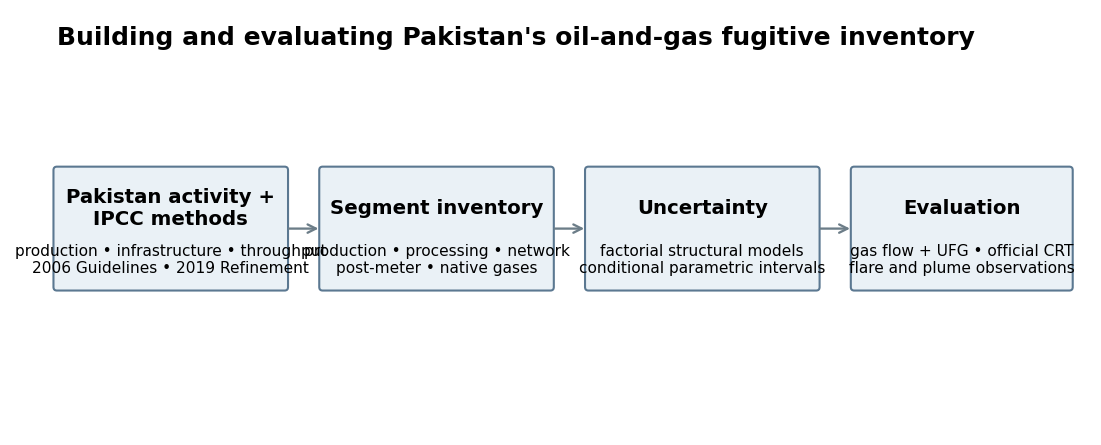
\includegraphics[width=0.90\textwidth]{fugitives_framework.png}
\caption{Scientific workflow from Pakistani activity data and IPCC methods through the segment
inventory, uncertainty analysis and three independent evaluation layers.}
\label{fig:framework}
\end{figure*}

% ===========================================================================
\section{Methodological context}
\label{sec:related}
% ===========================================================================

\subsection{From broad ranges to segment and practice factors}

The 2006 method was defensible when production was the only widely available activity, but its
developing-country ranges combine differences in source coverage, technology and practice. A
geometric midpoint can represent the centre of a bounded log interval; it cannot identify which
physical source is responsible for the result.

The 2019 Refinement changes that. For onshore gas production, for example, the methane factor is
\num{4.09} tonnes CH$_4$ per million m$^3$ for higher-emitting practices and
\SI{2.54}{} for lower-emitting practices, both with reported uncertainty of
$\pm\SI{20}{\percent}$. Distribution can be calculated from gas consumption or pipeline length
and is divided by plastic-pipeline and LDAR conditions. Transmission and processing similarly
distinguish LDAR and compressor-seal practice. Where these characteristics are unknown, the
guidance supports the higher-emitting/default selection and requires compilers to document it
\citep{ipcc2019}.

\subsection{Observation and inventory answer different questions}

Bottom-up and atmospheric estimates often disagree because average factors omit abnormal or
intermittent sources and because measurements sample different source populations. Aircraft and
facility synthesis in the United States found supply-chain methane materially above the national
inventory \citep{alvarez2018methane}; other work showed that a small, heavy-tailed source
population can reconcile apparently divergent estimates \citep{zavalaaraiza2015}. Large sources
also vary in time, so persistence cannot be inferred from a single overpass
\citep{cusworth2021intermittency}.

Satellite observations have made these releases independently visible. TROPOMI provides regional
methane sensitivity \citep{veefkind2012}; global analyses identify ultra-emitters
\citep{lauvaux2022} and national fossil-fuel corrections \citep{chen2023national}. Such
detections do not automatically produce annual national emissions: coverage, detection
thresholds, intermittency and attribution still matter. They can, however, test whether an
inventory's facility geography and source ranking are plausible. Global gridded fuel inventories
face the complementary problem of spatially allocating national reports
\citep{scarpelli2020,scarpelli2022}.

The same distinction applies to flare observations. The World Bank's Global Gas Flaring Tracker
derives annual flare volumes and individual flare locations from satellite radiance
\citep{worldbankflaring2026}. Because the 2019 production factors are inclusive of leakage,
venting and flaring, adding observation-derived flare emissions to them would double count.
Observed flaring is therefore retained as a memo and evaluation layer unless the inclusive
factor is first disaggregated.

\subsection{Official reporting as an audited comparator}

Pakistan's Biennial Transparency Report and CRT provide the authoritative national account
\citep{pakbtr2024,pakcrt2026}. Authority does not make a comparison scope-matched automatically.
The activity units, factors, notation keys, inventory year and GWP basis must be extracted and
compared explicitly. We treat the official submission as a comparator whose derivation is to be
reconstructed, not as a target to which the bottom-up model is forced.

% ===========================================================================
\section{Data and accounting boundaries}
\label{sec:data}
% ===========================================================================

\subsection{FY2015--16 to FY2023--24 infrastructure controls}

Oil and gas production come from the Pakistan Economic Survey 2025--26, which reports
\num{25.812} million barrels of crude oil and \num{1.141} million MMCF of natural gas in
FY2023--24 \citep{peseconomic2026}. Converted to IPCC activity units, these are
\num{4103.77} thousand m$^3$ of oil and
\num{32309.47} million m$^3$ of gas.

The Oil and Gas Regulatory Authority (OGRA) archive supplies annual refinery, network, customer,
consumption and UFG controls from FY2015--16 to FY2023--24
\citep{ograarchive,ogra2022,ogra2023,ogra2024}. Values are transcribed from the reported annual tables with
no interpolation. The image-based FY2020--21 report was independently OCR-audited against the
page images, and the FY2016--17 refinery total is retained as the regulator's restated value.
In FY2023--24, SNGPL reports
\SI{9320.69}{\kilo\metre} of transmission and
\SI{151419}{\kilo\metre} of distribution pipeline; SSGCL reports \SI{4206}{} and
\SI{49811}{\kilo\metre}, respectively. The combined systems serve \num{10748538} domestic,
\num{91925} commercial and \num{11318} industrial customers. Seventeen named compressor sites,
two LNG import terminals and \num{3437.13} MMCF d$^{-1}$ of utility and independent-system sales are
reported. The reference T\&D estimate uses measured pipeline length; throughput is an alternative
IPCC basis. Across the nine-year record, transmission length rises from
\SI{11555.08}{\kilo\metre} to \SI{13526.69}{\kilo\metre}, distribution length from
\SI{148278}{\kilo\metre} to \SI{201230}{\kilo\metre}, and domestic customers from \num{7997096} to
\num{10748538}. This supports a nine-year segment-resolved reconstruction rather than a
production-only historical extrapolation.

The FY2021--22 report identifies \SI{8200}{\kilo\metre} of polythene distribution pipe in the
SSGCL system. This is only \SI{4.2}{\percent} of the reported national distribution network and
does not classify the SNGPL network. Utility reports document active loss-control work---SNGPL
surveyed \SI{50250}{\kilo\metre} of underground network in FY2023--24 and both utilities report
rehabilitation and leak surveys---but do not establish national annual LDAR coverage
\citep{sngpl2024,ssgc2024}. Because the
2019 lower distribution factor requires both more than half plastic pipe and LDAR in use, the
public evidence does not resolve either national criterion sufficiently to select it.

OGRA reports \num{10.67} million tonnes of refinery product output. IPCC calls for crude feed,
so output converted at \SI{0.85}{\tonne\per\cubic\metre} is a provisional activity proxy with
\SI{20}{\percent} uncertainty. Produced gas is similarly used as provisional gas-processing
throughput. Neither proxy is hidden: both can be excluded by a coverage scenario.

Post-meter industrial activity is reconstructed directly from OGRA end-use controls rather than
one undifferentiated non-residential total. The included FY2023--24 classes are commercial,
general industry, fertilizer, captive power, cement and power stations, together
\num{2439.23} MMCF d$^{-1}$, which converts to \num{25211.03} million m$^3$ yr$^{-1}$;
the registered activity the leak factor rides is \num{25210.98} million m$^3$ yr$^{-1}$
before the fertilizer feedstock is withheld and \num{18684.62} after. The factor is defined
on gas consumed in combustion equipment, and \SI{83.5}{\percent} of the fertilizer class is
chemical feedstock, reformed and not burned, on the producers' metered feed and fuel gas
\citep{nfdc2025}; that feedstock, \num{6526.4} million m$^3$, is outside the base and the
process fuel stays in. Residential gas is
represented by the separate appliance fallback; CNG and unclassified other-system gas remain
outside the industrial/power row. The included class sum differs from the registered six-class
activity by only \num{0.042} million m$^3$ because published daily flows are rounded.

\begin{table*}[htbp]
\centering
\footnotesize
\begin{tabular}{@{}llrlp{6.0cm}@{}}
\toprule
\textbf{Segment} & \textbf{Activity} & \textbf{Value} & \textbf{Status} & \textbf{Principal structural issue} \\
\midrule
Oil production & onshore oil & 4,103.77 thousand m$^3$ & official & offshore split unavailable \\
Oil refining & converted product output & 12,552.94 thousand m$^3$ & proxy & crude-feed throughput unavailable \\
Gas production/gathering & produced gas & 32,309.47 million m$^3$ & official/proxy & well and field split unavailable \\
Gas processing & produced gas & 32,309.47 million m$^3$ & proxy & plant throughput and sour share \\
Transmission & pipeline length & 13,526.69 km & official & LDAR and seal practice \\
Distribution & pipeline length & 201,230 km & official & material share and LDAR \\
Post-meter appliances & domestic connections & 10,748,538 & official/proxy & one appliance per meter \\
Post-meter industry/power & non-residential gas & 25,210.98 million m$^3$ & official & factor transferability; fertilizer feedstock withheld from this base (see text) \\
\bottomrule
\end{tabular}
\caption{FY2023--24 reference activities. A proxy is estimated with an explicit fallback and
structural exclusion case; it is not described as observed.}
\label{tab:activity}
\end{table*}

\subsection{Observational and official comparison layers}

The current World Bank individual-flare workbook \citep{worldbankflaring2026}---built on
VIIRS Nightfire satellite pyrometry \citep{viirsnightfire}---contains annual volumes for
2012--2025 and \num{130} sites labelled Pakistan. The UNEP MARS snapshot contains plume and source tables under
a CC BY-NC-SA licence \citep{unepmars2026}; after filtering country and sector, it contains
\num{20} oil-and-gas sources and \num{174} plume detections. A public-domain geoBoundaries ADM1
layer assigns both products to provinces \citep{runfola2020}. Field-level evaluation uses
OGRA Table~3.34: its 84 published rows reconcile to \num{2637.75} MMCF d$^{-1}$, within
\num{0.03} MMCF d$^{-1}$ of the official total, and are canonicalized to 73 named fields.

The official comparison is extracted programmatically from Pakistan's 2022 CRT workbook. The
pipeline stores the package and workbook SHA-256 hashes, worksheet names, cell coordinates, raw
values, units, formulas and notation keys. The BTR's 2021 1.B.2 value is retained as a second
official-year comparator.

\subsection{Boundary and completeness}

The reference account covers oil and natural-gas systems under 1.B.2. Coal mining fugitives
(1.B.1) are outside the paper's stated boundary and are retained as NE in the completeness
matrix, now with a partial Tier-1 screen beside the key: the Thar mine-mouth deliveries the
power ledger holds bound the surface share (see
\texttt{outputs/fugitives\_coal\_screen\_2024.csv}), while underground production---whose
per-tonne factors run thirty times the surface low---remains unquantified. Oil and gas exploration, abandoned wells, natural-gas vehicles and anomalous events
also remain NE; storage is NO because the regulator describes facilities as planned rather
than operating. Venting and flaring are included elsewhere (IE) in the inclusive segment
factors and reported separately only as observation memos.
For every NE row, the completeness matrix records whether it is potentially material, probably
minor, unknown or outside scope and identifies the activity needed to estimate it. No numerical
upper bound is invented where public activity is unavailable.

% ===========================================================================
\section{Inventory construction}
\label{sec:methods}
% ===========================================================================

\subsection{Segment ledger and practice selection}

For segment $s$ and gas $g$, emissions are
\begin{equation}
E_{s,g}=A_s EF_{s,g}.
\end{equation}
Each ledger row carries the IPCC code, activity and unit, source and imputation status, factor,
uncertainty bounds and structural configuration. The accounting engine consumes this generic
schema, allowing facility records to replace aggregate proxies without changing the downstream
calculations.

The \emph{reference configuration} uses the higher/default 2019 practice factors where national
LDAR, pipeline-material or compressor-seal evidence is unavailable. Lower-practice factors and
throughput-based transmission and distribution are evaluated as structural alternatives.
Produced gas provides the processing proxy; sour-gas processing uses the 2019 default
\SI{32}{\percent} share. Both assumptions can be varied or excluded independently.

Post-meter appliances use one appliance per domestic meter and the Refinement's warm-country
fallback. The industrial/power factor is \SI{6.1}{\tonne} CH$_4$ per million m$^3$, derived in
the 2019 Refinement from a Revised 1996 value of \SI{175000}{\kilogram\per\peta\joule} and a
\SI{35}{\mega\joule\per\cubic\metre} gas conversion. Its older empirical basis motivates full,
half-factor and exclusion configurations. The complete factor lineage and uncertainty register
are given in the supplement.

\subsection{Method-resolution experiment}

Five estimates separate factor changes from boundary expansion:
\begin{enumerate}[leftmargin=*,itemsep=2pt]
\item the legacy 2006 production-only calculation for FY2019--20;
\item the same method on FY2023--24 production;
\item 2019 factors on identical FY2023--24 oil and gas production;
\item the 2019 upstream account after adding gathering and processing; and
\item the public-data 2019 ledger, including T\&D, LNG, refining and post-meter sources.
\end{enumerate}
The common-support comparison isolates the factor-framework effect; the later steps measure the
effect of representing additional physical segments.

\subsection{Monthly timing, upstream only}

The national release resolves this sector into fiscal months with process-specific support. Validated PBS provincial natural-gas and crude-oil production can support corresponding upstream production, gathering and processing timing as a throughput proxy. Twelve rows alone do not establish a complete national observation: source province coverage, units and compatible monthly or annual controls are checked against the final exported panel. Repaired extraction and worksheet selection are reflected in the current profiles. Where the source remains incomplete, an explicit fallback replaces the broken profile and carries weaker evidence; it is not labelled national observed activity.

Distribution, transmission, post-meter leakage and LNG follow deliveries or send-out, which are different physical drivers from field production. In the absence of appropriate observed monthly controls, those streams remain days-weighted or use a documented supported proxy. Refinery intake, wellhead production, flaring and venting retain distinct timing targets. The reference-year allocation does not imply observed changing geography across the extended annual series.

\subsection{Air-pollutant source boundaries}
The common source account supports admitted NMVOC and other pollutant factors for the specified oil/gas processes and flaring. Flaring combustion and venting are distinct, and factor coverage does not establish that every gas balance discrepancy is methane leakage. NH$_3$ and unresolved venting, post-meter or other pollutant categories remain notation gaps where no supported factor exists. The air ensemble reuses native fugitive activity realisations; an industrial gas-combustion draw deducts the same post-meter leakage quantity before applying a combustion factor.

\subsection{Process-matched allocation}

Production and gathering follow provincial oil and gas production. Transmission and
distribution follow measured pipeline length, post-meter industrial emissions follow gas
consumption, refineries follow facility output, and LNG terminals remain assigned to Sindh. Each
allocation reconciles exactly to its national control. Facility and network geometry is
insufficient for a defensible district grid, so the spatial product stops at process-matched
province and point layers.

The implementation tests unit exponents, source-row and segment closure, activity-year anchors,
pipeline and gas-flow identities, structural-model enumeration, uncertainty ordering,
observation coverage, official-inventory reproduction, provincial reconciliation and
manuscript-output agreement. Detailed assertions and generated products are documented in the
supplement and reproducibility appendix.

% ===========================================================================
\section{Uncertainty and physical controls}
\label{sec:uncertainty-controls}
% ===========================================================================

\subsection{Parametric uncertainty}

The legacy experiment samples each published 2006 factor from a bounded log-uniform
distribution and reports the median, P2.5, P97.5 and full methodological bounds. Rows in the
same physical stream share their range quantile.

For the 2019 inventory, published IPCC limits are interpreted as bounded expert ranges. A
split-triangular distribution places the reported value at the mode and median while preserving
the stated lower and upper limits. One production-volume deviate is shared across gas
production, gathering and processing; oil production and its transport fallback share the oil
deviate; and gases within a physical factor group share a quantile. Additional processing and
coverage residuals remain independent. The simulation uses \num{10000} iterations and seed 42.
The exact transformation, correlation groups and material inputs are reported in the supplement.

Input importance is measured by Spearman rank correlation with the national total. Normalized
squared correlations provide a screening measure of the parameters controlling the conditional
interval. A distribution-shape sensitivity reruns the reference model with bounded uniform and
bounded log-uniform inputs.

\subsection{Structural configurations}

The factorial experiment crosses upstream practice (higher/lower), network practice
(higher/lower), T\&D activity basis (pipeline length/throughput), post-meter industrial coverage
(fertilizer feedstock excluded, the reference/feedstock included/whole fertilizer class
excluded/half/excluded), processing activity (gross
production/marketable supply/excluded) and
sour-gas share (32\%/16\%/excluded). Removing invalid combinations leaves 280 deterministic,
unweighted configurations. No probability weights are assigned. We report one envelope for
models retaining every public-data
segment and a wider envelope that permits proxy-supported processing and post-meter coverage to
be excluded. A separate named \emph{central} configuration takes every stream with published
high/low practice bounds at their geometric mean; it is priced, never selected, and is not a
factorial leg because the practice bounds are readings of one control, not coverage choices.

Parametric intervals are calculated separately for five interpretable configurations:
reference, central, lower practices, no post-meter industrial/power, and the
minimum-coverage combined
case. This keeps uncertainty in measured activities and factors conditional on the selected
infrastructure model.

\subsection{Gas-flow balance and UFG diagnostic}

For each matched year, the physical account separates upstream and downstream identities:
\begin{align}
F_{gross}&=F_{indigenous,marketable}+R_{upstream},\\
F_{indigenous,marketable}+F_{RLNG}&=F_{use}+F_{UFG}+R_{downstream}.
\end{align}
The residuals preserve differences among published boundaries. The upstream disposition table
also records reinjection, own use, processing shrinkage, venting and flaring where public
quantities are available. Calendar-2024 VIIRS flare volume is shown as a volume-equivalent memo
against the adjacent gross-to-marketable difference.

UFG includes physical losses, theft, metering error and accounting effects. It is therefore used
only as a plausibility bound. If fraction $q$ were physical loss, the available methane would be
\begin{equation}
M_{\mathrm{CH_4}}=q V_{\mathrm{UFG}}\rho_{gas}x_{\mathrm{CH_4}}.
\end{equation}
Reference and lower-practice transmission-plus-distribution methane are expressed as the implied
fraction $q$; post-meter emissions are outside this utility balance.

% ===========================================================================
\section{External evaluation}
\label{sec:validation}
% ===========================================================================

\subsection{Official-inventory reconstruction}

Pakistan's 2022 Common Reporting Table (CRT) is evaluated first in native gases. Common-metric
comparisons use CO$_2$=1, fossil CH$_4$=30 and N$_2$O=265; the submitted total, which implies
CH$_4$=28, is also retained. A matched-year waterfall begins with the common-metric CRT, removes
separately reported venting and flaring already included in the 2019 Tier~1 factors, replaces
matched oil and gas categories, and adds public-data segments absent from the CRT. Every
published activity--factor product, native-gas subtotal and waterfall step is reproduced
programmatically. Adjacent FY2021--22 and FY2022--23 inventories bracket calendar 2022.

\subsection{Satellite and field evaluation}

World Bank flare volumes and UNEP MARS methane sources are joined to provincial boundaries and
to the 73 fields in the official gas-supply table. Each MARS source is assigned through its
nearest named flare; official fields without observations remain as zero-observation controls.
The evaluation reports marketable-supply coverage, Spearman and Kendall rank association, top-10
overlap, and national and within-province permutation tests for flare volume, MARS source count
and plume count. A match audit records distance, operator, canonical field and confidence for
every MARS source.

These observations evaluate upstream production and processing geography. Transmission,
distribution and post-meter sources require utility or facility measurements. Flare conversion
and MARS fluxes remain observational memos and do not enter the segment inventory.

\subsection{Evidence roles}

Table~\ref{tab:evidence} assigns each comparison a specific task. This separation prevents an
activity control, official account or intermittent observation from being treated as a universal
benchmark.

\begin{table*}[htbp]
\centering
\small
\begin{tabular}{@{}llll@{}}
\toprule
\textbf{Evidence} & \textbf{Question} & \textbf{Scale} & \textbf{Role} \\
\midrule
Gas-flow ledger & Are published supply and use controls compatible? & annual national & physical closure \\
UFG envelope & Is modelled network methane physically plausible? & annual utility & diagnostic bound \\
Pakistan CRT & Why does official reporting differ? & matched year/category & audited comparator \\
World Bank flares & Where is persistent combustion activity located? & field/site & spatial evaluation \\
UNEP MARS & Where are large detected methane sources? & event/field & spatial evaluation \\
Annual infrastructure controls & Does the reference result persist through time? & annual segment & temporal robustness \\
\bottomrule
\end{tabular}
\caption{Purpose and scale of the independent controls and comparisons.}
\label{tab:evidence}
\end{table*}

% ===========================================================================
\section{Results}
\label{sec:results}
% ===========================================================================

\subsection{Segment completion matters more than factor revision}

The legacy 2006 calculation is \SI{3.805}{\mega\tonne} \COe{} for FY2019--20 and
\SI{3.317}{\mega\tonne} on FY2023--24 production. Applying 2019 factors to the same FY2023--24
production raises the estimate to \SI{4.485}{\mega\tonne}. Adding gathering and processing
gives \SI{10.095}{\mega\tonne}; the full public-data ledger gives
\SI{23.499}{\mega\tonne}---high in the sector's \SIrange{9.601}{24.694}{\mega\tonne}
structural envelope, whose top keeps fertilizer feedstock inside the post-meter leak base
(Figure~\ref{fig:ladder}). The factor-framework
revision is therefore
smaller than the effect of representing additional supply-chain segments.

\begin{figure}[htbp]
\centering
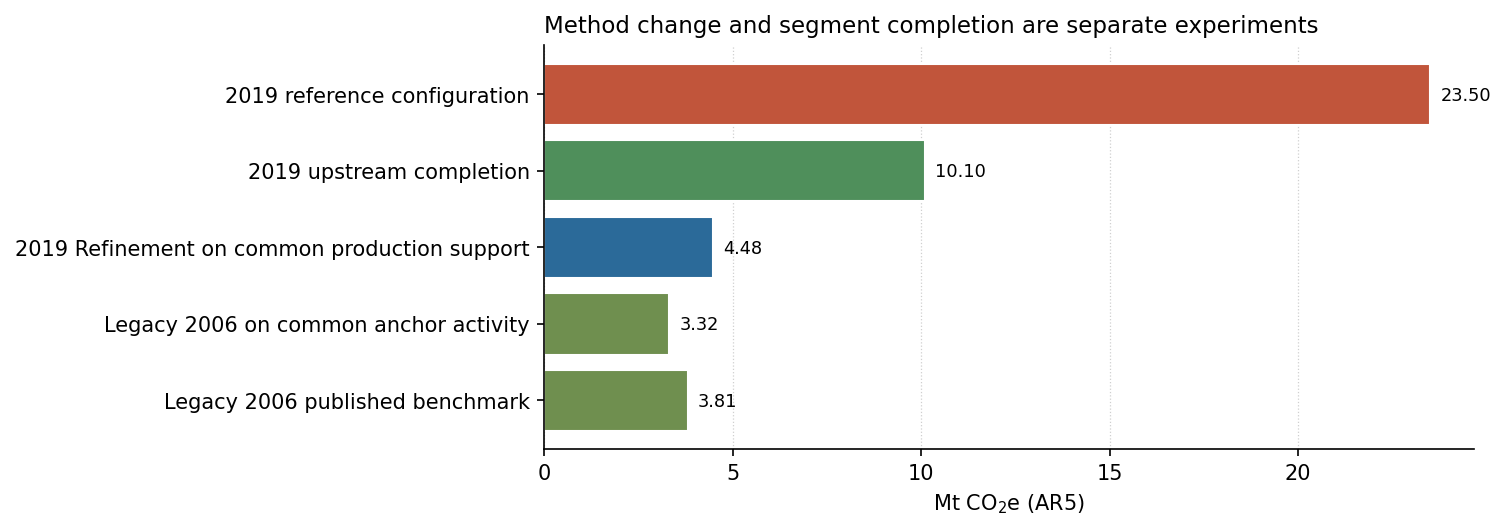
\includegraphics[width=\linewidth]{fugitives_method_ladder.png}
\caption{Method-resolution ladder. Common production support isolates the factor-framework
effect before the account expands to additional segments.}
\label{fig:ladder}
\end{figure}

\subsection{Distribution and post-meter assumptions determine the range}

The reference inventory contains \SI{752.761}{\giga\gram} CH$_4$,
\SI{915.619}{\giga\gram} CO$_2$ and \SI{3.483}{\tonne} N$_2$O
(Table~\ref{tab:segments}). Distribution is the largest segment
(\SI{7.069}{\mega\tonne}), followed by gas production (\SI{4.011}{\mega\tonne}),
post-meter industrial and power use (\SI{3.420}{\mega\tonne}) and gathering
(\SI{3.113}{\mega\tonne}).

\begin{table*}[htbp]
\centering
\scriptsize
\begin{tabular}{@{}lrrrrrl@{}}
\toprule
\textbf{Segment} & \textbf{CH$_4$ (Gg)} & \textbf{CO$_2$ (Gg)} & \textbf{N$_2$O (t)} &
\textbf{Mt \COe{}} & \textbf{Share (\%)} & \textbf{Activity} \\
\midrule
Gas distribution & 235.439 & 6.037 & 0.000 & 7.069 & 30.1 & official \\
Gas production & 132.146 & 46.849 & 0.808 & 4.011 & 17.1 & official \\
Post-meter industrial and power & 113.976 & 1.140 & 0.000 & 3.420 & 14.6 & official \\
Gas gathering & 103.390 & 11.308 & 0.194 & 3.113 & 13.2 & proxy \\
Gas processing & 59.126 & 3.877 & 0.042 & 1.778 & 7.6 & proxy \\
Gas transmission & 55.459 & 3.787 & 0.000 & 1.668 & 7.1 & official \\
Post-meter appliances & 34.395 & 0.344 & 0.000 & 1.032 & 4.4 & official \\
Sour-gas processing & 1.034 & 688.579 & 0.558 & 0.720 & 3.1 & IPCC default \\
Oil production & 14.076 & 50.887 & 0.780 & 0.473 & 2.0 & official \\
LNG import terminals & 3.320 & 29.374 & 0.000 & 0.129 & 0.5 & official \\
Oil refining & 0.377 & 73.435 & 1.101 & 0.085 & 0.4 & proxy \\
Oil pipeline transport & 0.022 & 0.002 & 0.000 & 0.001 & 0.0 & proxy \\
\midrule
\textbf{Total} & \textbf{752.761} & \textbf{915.619} & \textbf{3.483} &
\textbf{23.499} & \textbf{100.0} & \\
\bottomrule
\end{tabular}
\caption{Reference FY2023--24 inventory in native gases and AR5 CO$_2$ equivalent. Activity
status distinguishes official controls from proxy-supported rows. The reference total sits
high in the sector's 9.601--24.694~Mt structural envelope, whose top keeps fertilizer
feedstock inside the post-meter leak base.}
\label{tab:segments}
\end{table*}

\begin{figure}[htbp]
\centering
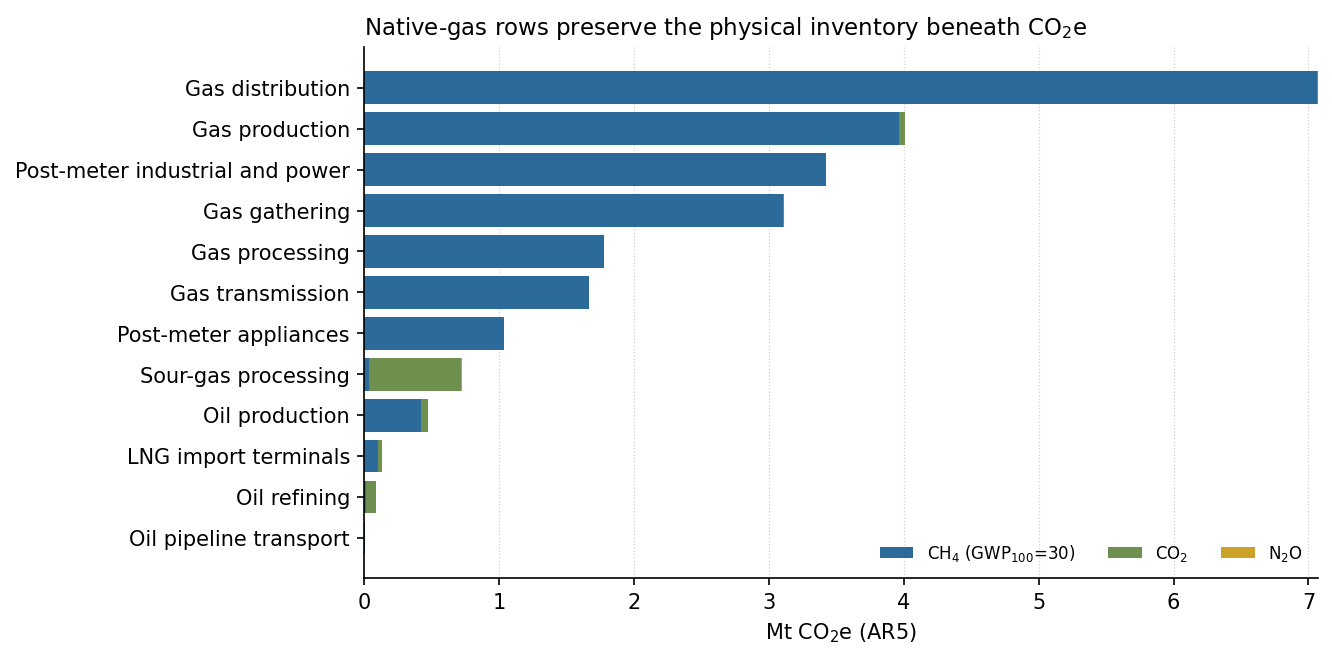
\includegraphics[width=\linewidth]{fugitives_streams.png}
\caption{Segment-level contributions by native gas.}
\label{fig:streams}
\end{figure}

The lower distribution factor reduces the national total by
\SI{5.679}{\mega\tonne}. Its selection requires more than half plastic pipe and active LDAR;
the publicly quantified \SI{8200}{\kilo\metre} of SSGCL polythene covers only
\SI{4.2}{\percent} of the national network. Halving or excluding the transferred post-meter
industrial/power factor reduces the total by \SI{1.710}{} or
\SI{3.420}{\mega\tonne}, respectively.

The named lower-practice configuration has a deterministic value of
\SI{14.894}{\mega\tonne}. A synthesized \emph{central} member---every stream with
published high/low practice bounds at their geometric mean, the retired 2006 method's
midpoint mechanism carried into the segment engine---prices \SI{17.678}{\mega\tonne},
with its own conditional interval of \SIrange{15.798}{21.309}{\mega\tonne}; it is a
named configuration, never the selection, because no measurement locates Pakistani
practice inside the bounds. The reference withholds the post-meter factor from the
fertilizer feedstock---gas chemically consumed in the reformers, not burned---and keeps the
plants' process fuel in the base. Putting the feedstock back inside the base, the membership
of earlier releases and one this paper does not defend, prices
\SI{24.694}{\mega\tonne} (the post-meter feedstock scope axis, \SI{+1.195}{\mega\tonne})
and is the top of the structural envelope; taking the
whole fertilizer class out prices \SI{23.264}{\mega\tonne} (\SI{-0.236}{\mega\tonne}).
Models retaining all public-data segments span
\SIrange{12.183}{24.694}{\mega\tonne} across the 192 segment-retaining members of the
280-configuration factorial. Permitting
proxy-supported processing and post-meter coverage to be excluded expands the envelope to
\SIrange{9.601}{24.694}{\mega\tonne}. The reference Monte Carlo has median
\SI{24.141}{\mega\tonne} and a 95\% interval of
\SIrange{21.277}{30.537}{\mega\tonne}. The national table prints the SAME
draws: the national Monte Carlo consumes this sector's persisted
\num{100000}-draw file (whose first \num{10000} draws are bit-identical to the run
above) and prints \num{24.15} for this module---the residual difference against
\num{24.141} is draw count, not convention. The 1.6-\si{\mega\tonne} family gap an
earlier edition had to explain away no longer exists;
\texttt{outputs/national\_uncertainty\_reconciliation.csv} now records the collapse. Corresponding intervals are
\SIrange{13.113}{17.311}{} for lower practices, \SIrange{18.489}{26.836}{} without industrial
post-meter emissions, and \SIrange{8.864}{10.692}{\mega\tonne} for the minimum-coverage case
(Figure~\ref{fig:uncertainty}).

\begin{figure*}[htbp]
\centering
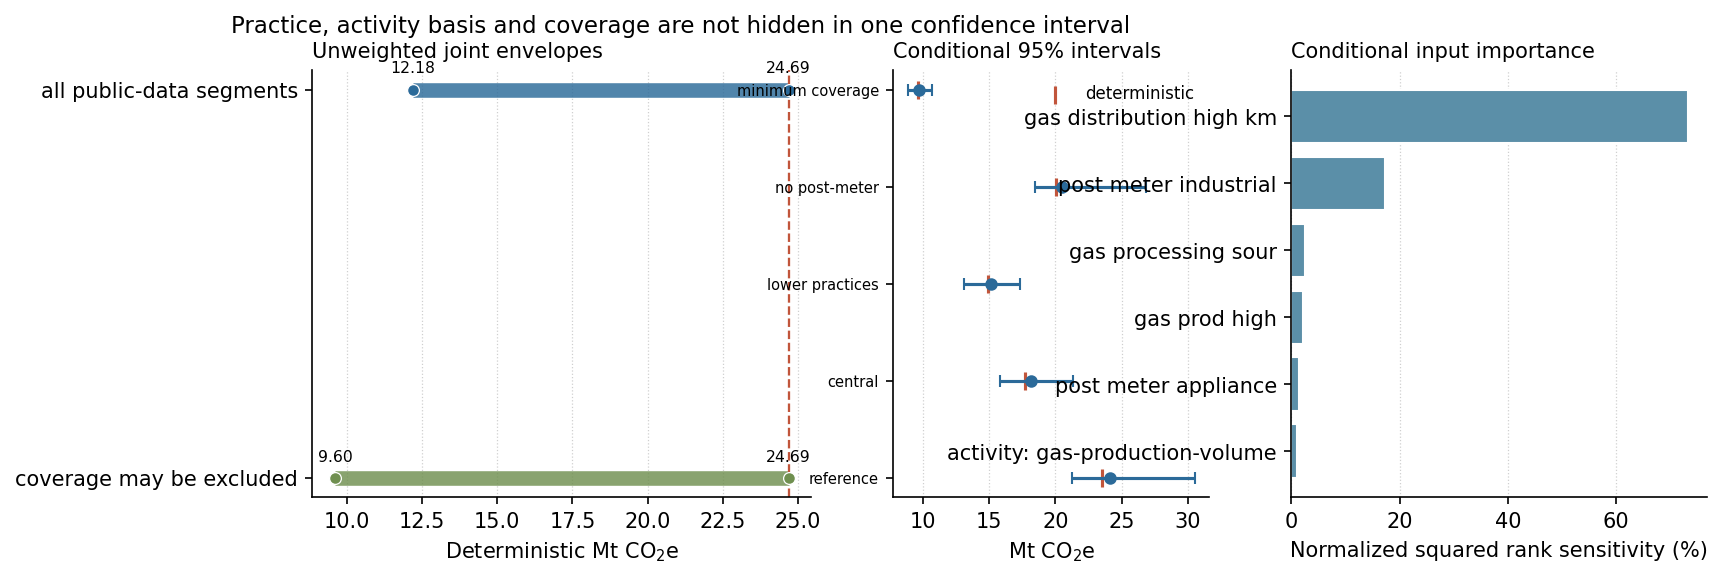
\includegraphics[width=0.96\textwidth]{fugitives_structural_uncertainty.png}
\caption{Structural envelopes, conditional parametric intervals and reference-configuration
input importance.}
\label{fig:uncertainty}
\end{figure*}

The distribution and post-meter factor groups contribute \SI{73.2}{\percent} and
\SI{17.2}{\percent} of normalized squared rank sensitivity, respectively. All remaining groups
individually contribute less than \SI{2.5}{\percent}. Alternative bounded distribution shapes
widen or shift the reference interval but leave these two measurement priorities unchanged
(Supplementary Table~S6).

\subsection{Network growth offsets declining upstream activity}

The public-data reconstruction ranges from \SI{24.384}{\mega\tonne} in FY2015--16 to a peak of
\SI{26.270}{\mega\tonne} in FY2018--19 and \SI{23.499}{\mega\tonne} in FY2023--24 (each
year's figure the reference configuration, feedstock outside the leak base in every year).
Its composition changes more clearly than its total. Upstream and processing emissions fall from
\SI{13.165}{} to \SI{10.181}{\mega\tonne} ($-22.7\%$), while network and LNG emissions rise
from \SI{6.698}{} to \SI{8.866}{\mega\tonne} ($+32.4\%$). Post-meter emissions remain nearly
constant at \SI{4.521}{} and \SI{4.453}{\mega\tonne}. Growth in pipeline length and customer
connections therefore offsets part of the decline in domestic production
(Figure~\ref{fig:official}, right).

\subsection{Physical balances and official reporting constrain magnitude}

Gross production exceeds indigenous marketable supply by \SI{11.4}{\percent}--
\SI{15.6}{\percent} across FY2021--22 to FY2023--24. The downstream balance is tighter:
indigenous marketable supply plus RLNG closes to reported supply, and the residual after
categorized consumption and UFG ranges from $-\SI{2.6}{\percent}$ to
$+\SI{1.4}{\percent}$.

Reference transmission-plus-distribution emissions are \SI{290.899}{\giga\gram} CH$_4$,
equivalent to \SI{23.8}{\percent} of reported UFG methane. Lower-practice estimates require
\SI{6.1}{\percent}; higher and lower throughput cases require \SI{18.8}{\percent} and
\SI{5.8}{\percent}. Both practice classes fit within the utility mass balance but imply sharply
different physical-loss shares (Figure~\ref{fig:ufg}).

\begin{figure*}[htbp]
\centering
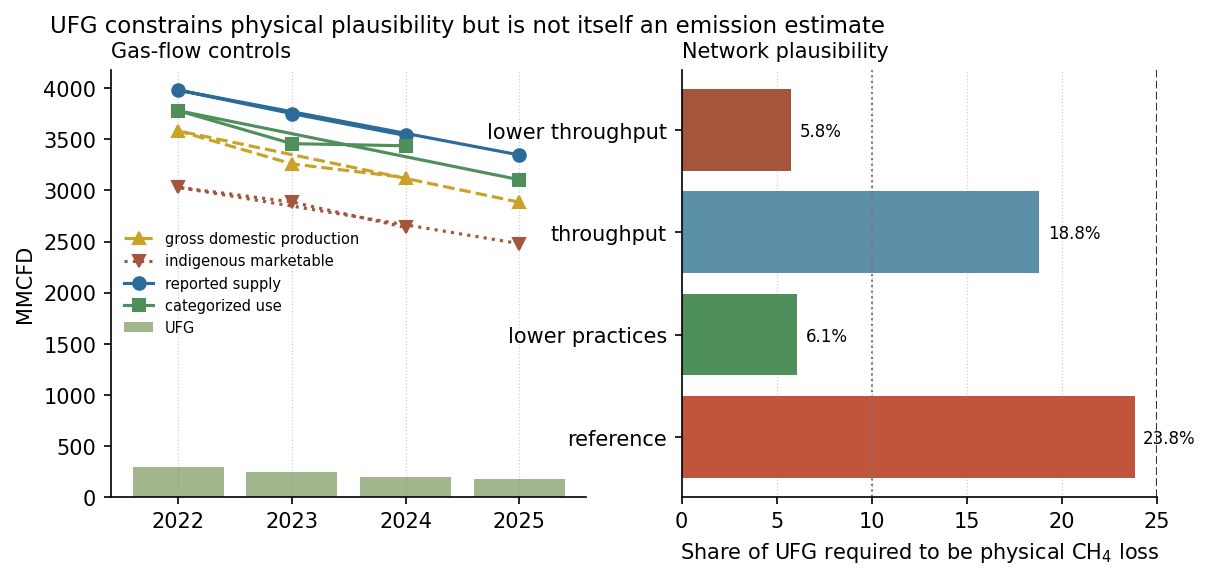
\includegraphics[width=0.94\textwidth]{fugitives_gas_flow_ufg.png}
\caption{Reported gas-flow controls (left) and the UFG share corresponding to modelled pre-meter
network methane (right).}
\label{fig:ufg}
\end{figure*}

Pakistan's 2022 CRT reports \SI{4.433}{\mega\tonne} for 1.B.2, or
\SI{4.749}{\mega\tonne} on the common GWP basis. The adjacent FY2021--22 and FY2022--23
reconstructions are \num{5.30} and \num{5.00} times this value. Fiscal-year choice changes the
reconstruction by about \SI{5.7}{\percent}.

Every CRT activity--factor row reproduces its reported native-gas result. The matched waterfall
then closes at \SI{25.187}{\mega\tonne} after harmonizing inclusive venting/flaring treatment,
replacing the oil and gas segment calculations, and adding LNG and post-meter sources. The
largest increments occur in gas production/gathering, processing, distribution and post-meter
activity (Figure~\ref{fig:official}, left).

\begin{figure*}[htbp]
\centering
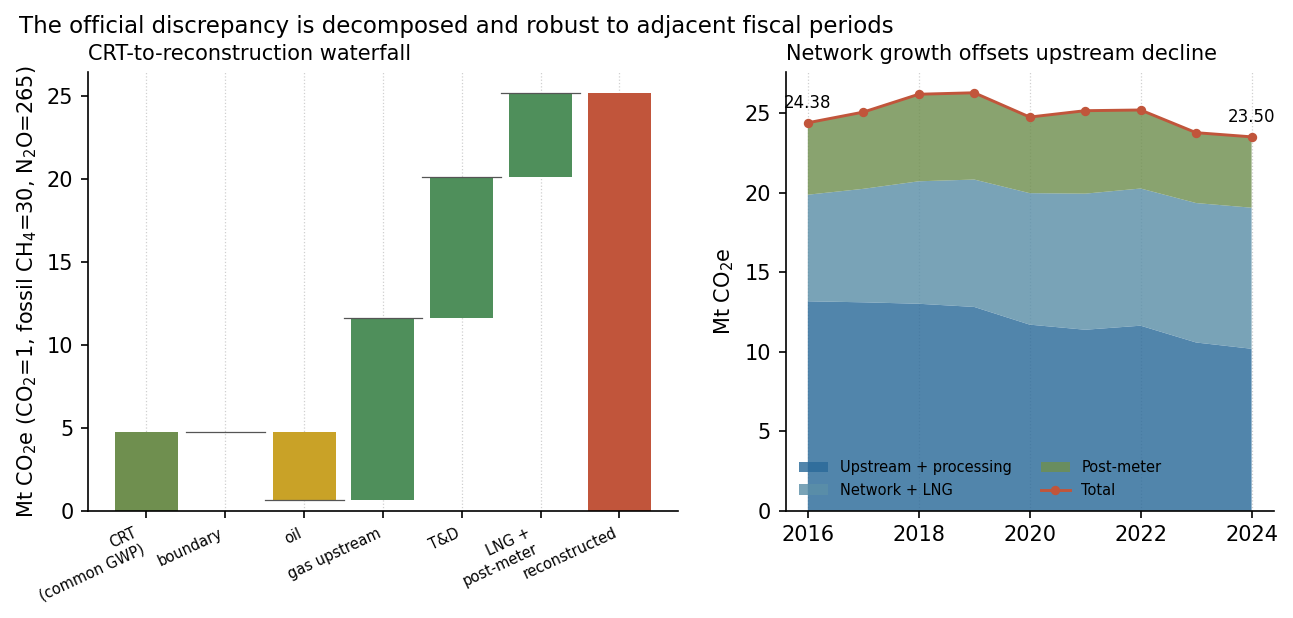
\includegraphics[width=0.95\textwidth]{fugitives_official_comparison.png}
\caption{CRT-to-reconstruction waterfall on a common GWP basis (left) and the segment-resolved
nine-year reconstruction (right).}
\label{fig:official}
\end{figure*}

\subsection{Production locates sources but weakly predicts observed intensity}

World Bank flare volume declines from \num{0.336} billion m$^3$ in 2012 to
\SI{0.130}{} in 2024. The MARS snapshot contains 20 oil-and-gas sources and 174 plumes;
19 sources occur within \SI{10}{\kilo\metre} of a World Bank flare. Matched detections occurred near
fields accounting for \SI{71.1}{\percent} of reported supply---a statement about where
the instruments matched, not about coverage: without sensor-opportunity, cloud and
detection-limit masks, a field with no matched event is unobserved, not observed-clean.

Across all 73 official fields, production has Spearman $\rho=\num{0.230}$ with VIIRS flare
volume and $\rho=\num{0.382}$ with MARS source and plume counts. Four fields overlap each
observation's production top-10. National and within-province permutations place the MARS rank
statistics at $p\leq\num{0.0013}$ and the corresponding top-field overlaps at
$p=\num{0.0065}$--$\num{0.0374}$. The VIIRS rank result is weaker, while its top-10 overlap is
less consistent with chance. Production therefore identifies broad upstream geography but
explains little of the observed intensity variation (Figure~\ref{fig:observations}).

\begin{figure*}[htbp]
\centering
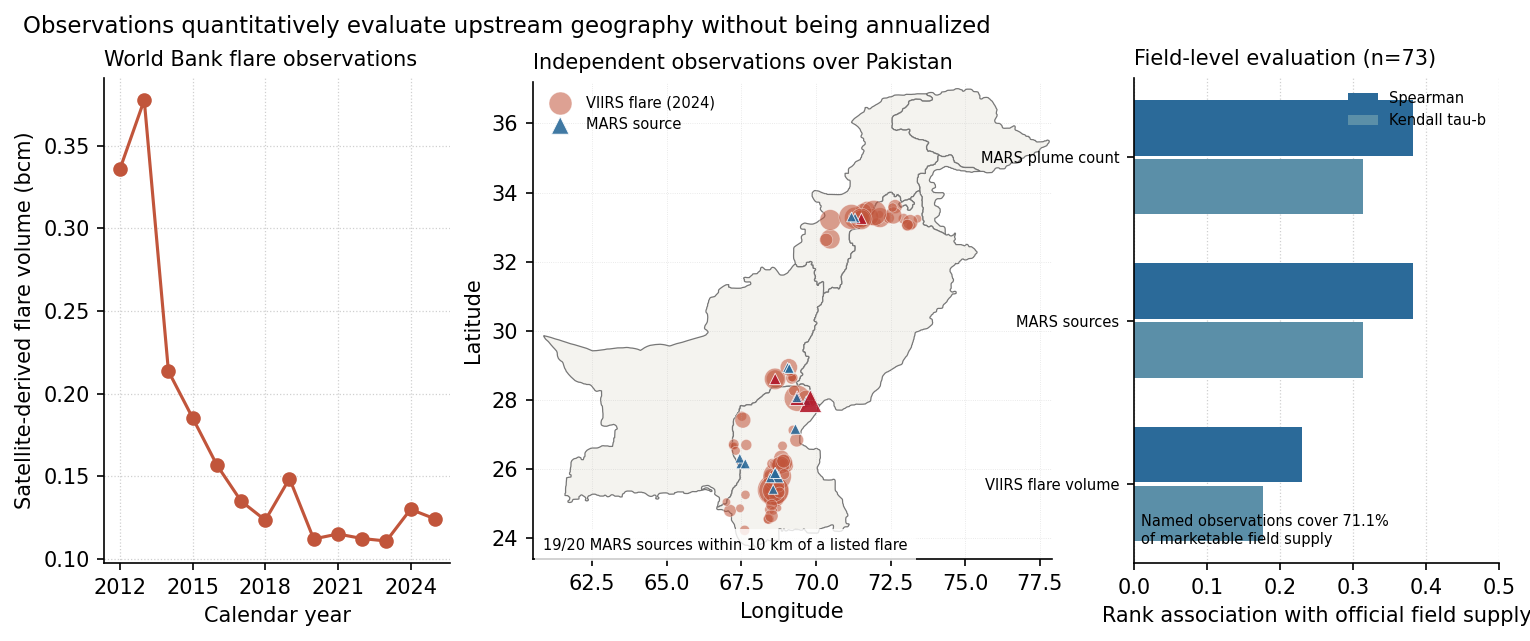
\includegraphics[width=0.95\textwidth]{fugitives_observations.png}
\caption{Annual flare volume, mapped field/flare/MARS observations and field-level ranking
diagnostics.}
\label{fig:observations}
\end{figure*}

The process-matched provincial inventory is \SI{9.99}{\mega\tonne} in Sindh,
\SI{7.77}{} in Punjab, \SI{2.86}{} in Khyber Pakhtunkhwa,
\SI{2.79}{} in Balochistan and \SI{0.09}{} in Other.

% ===========================================================================
\section{Discussion}
\label{sec:discussion}
% ===========================================================================

\subsection{Segment completion changes national accounting}

The common-support experiment identifies a modest increase from the 2006 to the 2019 production
factors. The much larger change appears when gathering, processing, network and post-meter
sources enter the account. For data-scarce countries, applying a newer production factor while
retaining a production-only boundary would therefore capture only a small part of the
Refinement's effect.

The segment-resolved reconstruction reinforces this interpretation. Domestic gas production declines,
but distribution length and customer connections grow. The resulting shift from upstream to
network emissions leaves the national total comparatively stable. A production-scaled time
series would miss that structural change and direct mitigation attention toward a shrinking
share of the system.

\subsection{Two infrastructure questions define the national range}

Distribution practice and post-meter industrial leakage determine most of both the structural
range and the reference-configuration sensitivity. National pipe material, pressure, age and
annual LDAR coverage would establish whether Pakistan meets the lower distribution-factor
criteria. Public utility reports confirm ongoing leak surveys and rehabilitation, but the
quantified material evidence covers only a small part of the network.

The industrial/power factor presents a different problem. Its IPCC lineage and unit conversion
are explicit, and national activity is available by end-use class, but its empirical technology
population comes from an older global default. The full, half-factor and exclusion cases show
the consequence of that transfer. Measurements at power stations, general-industry sites
and captive-power facilities would address the largest end-use components directly.

The reference configuration provides a reproducible application of the public evidence. The
factorial envelopes show how alternative practice, activity-basis and coverage choices affect
that result, while the conditional intervals quantify uncertainty within named configurations.
Together they identify the observations capable of reducing uncertainty instead of compressing
all model choices into one percentage.

\subsection{Utility and official accounts identify reconciliation priorities}

The gas-flow ledger establishes a coherent downstream system from indigenous marketable supply
and RLNG to categorized use and UFG. Its unresolved upstream residual highlights a separate data
need: plant throughput, reinjection, own use, processing shrinkage and operator venting/flaring.
Those quantities would also improve the processing activity basis.

The UFG comparison translates network estimates into a quantity utilities can test. The
reference and lower-practice configurations require markedly different physical shares of the
reported balance, creating a direct role for utility loss audits that separate leakage from
theft, metering and billing effects.

The CRT reconstruction locates the official difference in source representation. Common GWP
conversion and adjacent fiscal years remove metric and period alignment as major explanations;
the public workbook itself is arithmetically coherent. The waterfall instead points to gas
production/gathering activity, processing, distribution, post-meter coverage and the oil--gas
allocation. Reconciliation should therefore begin with the underlying activity bridge and
category boundaries.

\subsection{Satellite observations reveal heterogeneous upstream emissions}

The field analysis supports the broad geography of the upstream inventory while challenging a
simple production-intensity relationship. Observations cover most reported marketable supply,
and MARS source locations are non-random with respect to producing fields. Their modest rank
association with production is consistent with equipment, operating practice and intermittent
events controlling emissions at individual sites.

This finding has two implications. First, production remains useful for allocating an aggregate
upstream estimate when facility activity is incomplete. Second, production cannot substitute
for facility observations when identifying high emitters. Repeated plume coverage, plant and
compressor inventories, and operator-matched field data would turn the present geographic test
into a stronger facility-level evaluation.

\subsection{Implications for data-scarce inventories}

The source-neutral ledger makes future improvements local. Well and field records can replace
national production proxies; plant throughput can resolve processing and disposition; utility
material and pressure classes can select network factors; and facility measurements can replace
transferred post-meter factors. The evidence ranking indicates that national distribution
technology, post-meter measurements and upstream disposition should precede refinements to minor
oil-transport or LNG rows.

More generally, the study shows why factor selection, boundary completion and evaluation should
be treated as separate tasks. A newer factor framework improves an inventory only when its
physical segments are represented, while independent controls are most informative when matched
to the processes they can observe.

% ===========================================================================
\section{Limitations}
\label{sec:limitations}
% ===========================================================================

Pakistan-specific equipment and leakage measurements remain sparse. National pipe material,
pressure class, network age, annual LDAR coverage, compressor type and seal configuration were
unavailable. The post-meter industrial/power factor is transferred from the IPCC default, and
processing uses produced or marketable gas in the absence of plant throughput. These inputs
control the largest structural differences.

The post-meter factor also rides gas the combustion sectors meter: the national
gas ledger (\texttt{outputs/national\_gas\_closure.csv}) joins OGRA Table~3.31's end-use
partition to each consuming module's live quantity and quantifies the leaked share of
the burned-and-leaked classes' double-claim at about \SI{1.0}{\percent} of their
whole-gas mass. The combustion side books its gas rows \emph{net}
of that share, so no molecule is claimed both burned and leaked, and this sector's leak claim
is unchanged. The gross delivered-gas booking is the joint national configuration
\emph{gross\_delivered\_gas\_accounting}
(\SI{+0.288}{\mega\tonne} of combustion \COtwo{}e restored onto the gas rows the
consuming modules book net; \texttt{outputs/national\_gas\_closure\_variant.csv}). That figure is the combustion side of the four burned streams
and holds no fertilizer term. Fertilizer gas is the ledger's sharpest single class,
\SI{31}{\percent} of the six classes the leak base is drawn from, and it is carried as two
rows. The chemical feedstock, \SI{83.5}{\percent} of the class, is reformed and not burned:
it sits outside every combustion module and outside the leak base. The
process fuel is burned at the plants and stays inside it. A membership with the
feedstock inside the base is published as the scenario
\emph{post\_meter\_including\_feedstock} (\SI{24.694}{\mega\tonne}), the highest case of the
structural envelope; it carries no probability and is not the reference.

The public gas-flow account does not resolve reinjection, own use, processing shrinkage or
operator venting and flaring. Active and abandoned wells, exploration, workovers, pneumatic
equipment, blowdowns, accidents and anomalous releases remain NE or embedded in inclusive
factors according to the completeness matrix. A complete well-, facility- and component-level
ledger would improve both coverage and technology classification.

Satellite evidence is spatially and temporally selective. VIIRS detects combustion radiance,
MARS emphasizes large intermittent plumes, and only \num{8} of the \num{73} official fields
receive matched MARS events. A zero in the matched record is therefore not an observed
non-detection: it may be unobserved, cloud- or geometry-limited, below the detection
threshold, or outside sensor coverage, and the permutation tests retain those zeros as
rank evidence only---no field is read as observed-clean. Building the sensor-opportunity
cube that would separate these cases is named future work. The field analysis
consequently tests upstream geography; network and post-meter rows
need utility, facility or urban atmospheric measurements.

The full infrastructure reconstruction begins in FY2015--16, and fiscal years only bracket the
calendar-2022 CRT comparison. Structural envelopes cover the declared public-data choices but
cannot enumerate every physical configuration. Conditional intervals also depend on the bounded
input distributions documented in the supplement.

% ===========================================================================
\section{Conclusion}
\label{sec:conclusion}
% ===========================================================================

On common FY2023--24 production support, the legacy and refined methods give
\SI{3.317}{} and \SI{4.485}{\mega\tonne} \COe{}. Expanding to the public-data 2019 segment
ledger raises the conservative (default-practice) configuration to
\SI{23.499}{\mega\tonne}---high in its own 9.601--24.694 joint envelope, whose top is the
same practice setting with fertilizer feedstock inside the post-meter leak base. The
reference should be read as an
upper-practice conservative configuration and never as an empirically centred
best estimate: no probability attaches to any point in the envelope, and until
Pakistani pipe-material, pressure, LDAR or post-meter measurements exist, the
honest statement is the envelope with its selection rule, with the joint floor
priced beside it. The principal change is
therefore supply-chain coverage rather than the production-factor revision alone.

Joint structural choices span \SIrange{9.601}{24.694}{\mega\tonne}. Distribution technology
and transferred post-meter industrial leakage determine most of this range and
\SI{90.4}{\percent} of the reference-configuration rank sensitivity. Utility balances show that
the network estimates are physically feasible, while distinguishing sharply between higher- and
lower-practice interpretations.

Both adjacent-fiscal-year bracket endpoints are more than five times Pakistan's 2022 CRT
on a common GWP basis;
the difference traces to activity, factor and boundary choices rather than arithmetic. Satellite
observations confirm broad upstream source geography but show that production weakly predicts
detected intensity. National pipe characteristics, post-meter measurements and plant gas
disposition are therefore the highest-value next data. The implemented ledger can incorporate
those records without another methodological redesign.

\FloatBarrier

% ---------------------------------------------------------------------------
\section*{Code and data availability}
% ---------------------------------------------------------------------------

The calculation engine, the activity data and every output quoted here are version-controlled
in the inventory repository (\url{https://github.com/PakAirQuality/pakistan-emissions-sectors})
and reproduce from a single command. The sector is regenerated with
\texttt{python3 -m pkinv.sectors.fugitives.run\_fugitives}; \ref{app:repro} gives the full
sequence. Every number printed in this paper is read from a generated CSV rather than
transcribed, and a test asserts that the manuscript and the engine agree.

% ---------------------------------------------------------------------------
\bibliographystyle{elsarticle-harv}
\bibliography{../../paper_common/references}

% ---------------------------------------------------------------------------
\appendix
\renewcommand{\thetable}{\arabic{table}}%
\renewcommand{\thefigure}{\arabic{figure}}%
% ===========================================================================
\section{Reproduction and generated products}
\label{app:repro}
% ===========================================================================

The inventory is regenerated from the repository root with:

\begin{verbatim}
pip install -e .
python3 -m pkinv.sectors.fugitives.run_fugitives
python3 -m pkinv.report.figures
python3 scripts/sync_figures.py
python3 -m unittest discover -s tests
\end{verbatim}

The runner writes the evidence tables below. Each is named: the registered filenames use the
FY2023--24 anchor suffix \texttt{2024}, and stating the convention without stating the names
left a reader unable to tell which file was which. Every quantity this paper prints from one of
them is checked against it by the verification registry.

\begin{itemize}\itemsep2pt
\item \texttt{fugitives\_\allowbreak segment\_\allowbreak native\_\allowbreak gases\_\allowbreak 2024.csv}: the segment ledger in native
  gases: \CHfour{}, \COtwo{} and \NtwoO{} for each of \num{12} segments, with each segment's
  share of the sector.
\item \texttt{fugitives\_method\_ladder\_2024.csv}: the method ladder, ordered, each rung
  with its coverage and result.
\item \texttt{fugitives\_\allowbreak structural\_\allowbreak factorial\_\allowbreak 2024.csv}: all \num{280} factorial
  configurations of the practice, basis and sour-fraction choices.
\item \texttt{fugitives\_\allowbreak structural\_\allowbreak scenarios\_\allowbreak 2024.csv}: the named structural
  experiments, each with its activity basis and practice.
\item \texttt{fugitives\_\allowbreak conditional\_\allowbreak intervals\_\allowbreak 2024.csv}: \num{5} conditional Monte
  Carlo intervals, one per configuration, beside that configuration's deterministic value.
\item \texttt{fugitives\_\allowbreak uncertainty\_\allowbreak attribution\_\allowbreak 2024.csv}: rank attribution by input
  group, as normalised squared Spearman correlation.
\item \texttt{fugitives\_\allowbreak infrastructure\_\allowbreak timeseries\_\allowbreak 2016\_\allowbreak 2024.csv}: the \num{9}-year
  infrastructure reconstruction.
\item \texttt{fugitives\_\allowbreak infrastructure\_\allowbreak segment\_\allowbreak timeseries\_\allowbreak 2016\_\allowbreak 2024.csv}: the same
  years decomposed by segment.
\item \texttt{fugitives\_\allowbreak gas\_\allowbreak flow\_\allowbreak balance\_\allowbreak 2022\_\allowbreak 2024.csv}: the gas-flow balance: gross
  domestic production, indigenous marketable supply and the upstream statistical difference
  between them.
\item \texttt{fugitives\_\allowbreak ufg\_\allowbreak network\_\allowbreak compatibility\_\allowbreak 2024.csv}: the UFG test---the
  physical fraction each scenario would require, and whether it is compatible with a
  \SI{10}{\percent} and a \SI{25}{\percent} unaccounted-for-gas figure.
\item \texttt{fugitives\_\allowbreak post\_\allowbreak meter\_\allowbreak end\_\allowbreak use\_\allowbreak 2024.csv}: post-meter throughput by end
  use, with the IPCC inclusion decision for each.
\item \texttt{fugitives\_\allowbreak post\_\allowbreak meter\_\allowbreak factor\_\allowbreak lineage\_\allowbreak 2024.csv}: that factor's lineage
  from its published value to the registered one, rounding difference included.
\item \texttt{fugitives\_\allowbreak distribution\_\allowbreak practice\_\allowbreak evidence\_\allowbreak 2024.csv}: the evidence that
  classifies the distribution network, each item with its criterion, coverage and effect on the
  classification.
\item \texttt{fugitives\_\allowbreak observation\_\allowbreak field\_\allowbreak statistics\_\allowbreak 2024.csv}: field-level agreement
  with the satellite observations.
\item \texttt{fugitives\_\allowbreak observation\_\allowbreak permutation\_\allowbreak 2024.csv}: the permutation tests that
  give that agreement an empirical \emph{p}.
\item \texttt{fugitives\_data\_priorities\_2024.csv}: which input or decision would move
  the answer most, ranked by effect.
\item \texttt{fugitives\_benchmark\_crosswalk.csv}: the external comparators on a common
  GWP basis, each with its independence from this inventory recorded.
\item \texttt{fugitives\_mars\_summary.csv}: the MARS plume summary---sources, plumes,
  persistent and notified counts and the maximum observed flux.
\item \texttt{fugitives\_viirs\_flare\_sites.csv}: the flare-site register, with each
  site's volume per year.
\item \texttt{fugitives\_\allowbreak viirs\_\allowbreak flaring\_\allowbreak 2012\_\allowbreak 2025.csv}: the national series of flared
  volume and active site count.
\end{itemize}

The sector's headline tables are the seven below. They were described in this appendix by
function---``the process-matched provincial allocation'', ``the completeness matrix''---and
named nowhere, which tells a reader that the evidence exists without telling them where it is.

\begin{itemize}\itemsep2pt
\item \texttt{fugitives\_totals\_2024.csv}: the registered sector result, by category and
  method, with the fiscal year, the AR5 total and the Monte Carlo 2.5th, 50th and 97.5th
  percentiles beside it.
\item \texttt{fugitives\_\allowbreak by\_\allowbreak stream\_\allowbreak 2024.csv}: the stream ledger---category,
  subitem and gas in gigagrams, each row with its uncertainty, correlation group,
  fossil flag, activity year and period kind, evidence class, and temporal and spatial method.
\item \texttt{fugitives\_provincial\_2024.csv}: the province-level AR5 total.
\item \texttt{fugitives\_monthly\_2024.csv}: the twelve-month layer, each month's share with
  the emissions it implies in both common-GWP vintages, and the temporal method and basis that
  produced the shape.
\item \texttt{fugitives\_\allowbreak completeness\_\allowbreak 2024.csv}: one row per IPCC code and subsegment
  with its notation key, treatment, principal gap, materiality class and screening bracket.
\item \texttt{fugitives\_\allowbreak uncertainty\_\allowbreak 2024.csv}: per segment, the mean and the 2.5th,
  50th and 97.5th percentiles with the observed minimum and maximum, and the method,
  scenario, distribution, iteration count and seed that generated them.
\item \texttt{fugitives\_\allowbreak observation\_\allowbreak provincial\_\allowbreak evaluation\_\allowbreak 2024.csv}: the
  provincial confrontation of the upstream inventory with the observations---flared volume,
  active and total flare sites, and MARS source and plume counts, persistent ones separately.
\end{itemize}

The runner also writes the reference component table, the auditable site matches, the CRT
extraction, the common-GWP waterfall, the row reproduction and cell audit, the QA table and the
run manifest. The legacy FY2019--20 calculation remains a labelled row rather than the
registered sector result.

The run manifest records each input path and SHA-256 hash. Tests assert the registered year,
matched-year activity conversion, IPCC factor identity, alternative activity bases, gas-flow
identities, no duplicate segment--gas rows, uncapped bounded legacy sampling, shared uncertainty
groups, UFG exclusion and compatibility, quantitative observation coverage, CRT row closure,
provincial reconciliation and source-status notation.

% ===========================================================================
\section{Factor and activity audit}
\label{app:factors}
% ===========================================================================

The machine-readable factor registry is
\path{data/fugitives_ipcc2019_factors.csv}. Each row stores its 2019 Refinement table,
activity unit, reported factor, lower and upper uncertainty, practice class and correlation group.
The legacy factors remain in \texttt{data/emission\_factors.csv} only for the method benchmark.

Reference activities are stored in
\path{data/activity/fugitives/anchor_activity_2023_24.csv} and the matched-year extension in
\path{data/activity/fugitives/anchor_activity_2021_23.csv}. Historical controls are in
\path{data/activity/fugitives/infrastructure_history_2015_21.csv}; field, distribution-practice
and post-meter audits have separate source tables in the same directory. Official quantities and
fallbacks are distinguished in the \texttt{method\_tier}, \texttt{status} and \texttt{note}
fields. The factor engine accepts this generic schema; it does not read OGRA or satellite files
directly.

The official-inventory audit exports the workbook filename and package hash, worksheet, cell or
range, raw value, unit, formula where present, notation key and extraction transformation. This
is intended to make the reported oil--gas allocation independently checkable rather than to
infer unpublished institutional reasoning.

The complete uncertainty-input register, including distributions, bounds and shared deviates,
is reproduced as Table~S5 in the supplementary material. The machine-readable source remains
\path{outputs/fugitives_uncertainty_inputs_2024.csv}.

% ===========================================================================
\section{Notation keys and import contract}
\label{app:completeness}
% ===========================================================================

Completeness follows the UNFCCC notation convention: \emph{estimated} identifies ledger rows,
IE identifies quantities included elsewhere in an inclusive factor, NE identifies categories
for which evidence is not yet sufficient, and NO identifies activities documented as not
occurring. Venting and flaring are IE in the reference Tier~1 production factors; the VIIRS result
is consequently a memo, not an additional stream.

Table~S4 in the supplementary material reproduces the complete notation-key and materiality
matrix, including the activity evidence required to replace every NE entry. The observation
join audit and its 10,000-draw permutation diagnostics are given in Tables~S1--S3.

The permanent import contract for future PPIS, OGRA or operator records requires a source
identifier, reporting period, IPCC segment, facility or network identifier, operator, location,
activity value and unit, technology/practice class, source reference, imputation method and
quality flag. Missing records remain explicit residuals. Facility observations may replace an
aggregate activity row or evaluate its geography, but they cannot silently change the inventory
boundary or force closure.

% ===========================================================================
\section{Legacy uncertainty experiment}
\label{app:legacy}
% ===========================================================================

For the 2006 benchmark, a published factor range $[L,U]$ is sampled directly as
\begin{equation}
EF=\exp\left[\ln L+q(\ln U-\ln L)\right],\qquad q\sim\mathcal{U}(0,1).
\end{equation}
All gases in one physical stream share $q$. The geometric midpoint is therefore the median of
the factor distribution, every draw remains within the published bounds, and no display or
computational cap is applied. This bounded log-uniform experiment is retained only to diagnose
the legacy method; it is not the uncertainty model used for the 2019 segment inventory.


\end{document}
